\documentclass{llncs}

%\usepackage{llncsdoc}

%\usepackage{makeidx}  % allows for indexgeneration
\usepackage{graphicx}
\usepackage[T1]{fontenc}
\usepackage[english]{babel}
\usepackage[utf8]{inputenc}

\usepackage{paralist}


%%%Math
\usepackage{latexsym}
\usepackage{amsmath}
\usepackage{amssymb}
\usepackage{amsthm}

\usepackage{algorithm}
\usepackage{algorithmic}

\usepackage{longtable}

\usepackage{listings}

\usepackage{color}

\definecolor{darkred}{rgb}{0.5, 0, 0}
\definecolor{violet}{rgb}{1, 0, 1}
\definecolor{green}{rgb}{0.3, 0.95, 0.3}
\definecolor{listinggray}{gray}{0.97}

\lstset{
	basewidth=0.45em,
	backgroundcolor=\color{listinggray},
	basicstyle=\footnotesize\ttfamily,
	breaklines=true,
	keywordstyle=\bfseries,
	stringstyle=\itshape,
	commentstyle=\itshape,
	showspaces=false,
	showtabs=false,
	showstringspaces=false,
	frame=trbl,
	frameround=tttt,
	extendedchars=true,
	numbers=none,
	aboveskip=0.5cm,
	belowskip=0.5cm,
	xleftmargin=0cm,
	xrightmargin=0cm
}


\begin{document}

\title{ONTOSPREAD: Activation of Concepts in Ontologies through the Spreading
Activation algorithm}

\titlerunning{ONTOSPREAD: Activation of concepts in ontologies through the
Spreading Activation algorithm}

\author{Jose Mar\'{i}a \'{A}lvarez\inst{1} \and Diego Berrueta\inst{2} \and Luis Polo
\inst{2} \and Jos\'{e} Emilio Labra\inst{1}} 


\authorrunning{Jose Mar\'{i}a Alvarez et al.}


\tocauthor{Jose Mar\'{i}a \'{A}lvarez, Diego Berrueta, Luis Polo, Jos\'{e} Emilio
Labra} 


\institute{WESO RG, Universidad de Oviedo, Oviedo, Asturias, Spain,\\
\email{\{josem.alvarez,jelabra\}@weso.es},\\ 
 WWW home page: \texttt{http://www.weso.es}
\and
Fundación CTIC, Gij\'{o}n, Asturias, Spain,\\
\email{\{diego.berrueta,luis.polo\}@fundacionctic.org},\\ 
 WWW home page: \texttt{http://www.fundacionctic.org}
}

\maketitle

\begin{abstract}
The present article introduces the ONTOSPREAD API for the development,
configuration, customization and execution of the Spreading Activation
techniques over semantic networks and more specifically over RDF graphs and ontologies 
arising from the Semantic Web area. These techniques have been used to
the efficient exploration and querying of large and heterogenuos knowledge bases 
based on semantic networks in the Information or Document Retrieval domains. 
ONTOSPREAD implements the double process of activation and spread of concepts in ontologies, implicit
graph structures, applying different restrictions of the original model like weight degradation 
according to the distance or others comming from the extension of these techniques like
the converging paths reward. The main application of Spreading Activation
lies in two different areas of interest to digital libraries: 1) construction of hybrid semantic search engines 2) ranking of
information resources according to an input set of weighted resources. These techniques provide a whole framework to ease
the information access, a common required features in the exploitation
of new and existing digital libraries. Finally, in this work an evaluation methodology and 
an example using the Galen ontology are provided to validate the goodness, the improvement and the capabilities of 
this framework applied to digital libraries.
\end{abstract}

\section{Introduction}
The Spreading Activation technique (hereafter SA) introduced by~\cite{Collins_Loftus_1975}, in the field of 
psycho linguistics and semantic priming, proposes a model in which all relevant information is mapped
on a graph as nodes with a certain ''activation value``. Relations between two concepts
are represented by a weighted edge. If a node is activated their activation value is spread
to their neighbor nodes. This technique was adopted by the computer science community and applied
to the resolution of different problems, see Sect.~\ref{related-work}, and it is relevant to
the medical fields sector in the scope of: 1) construction of hybrid semantic search engines;  2) ranking of
information resources according to an input set of weighted resources 3) recommendation of medical terms using
well-known ontologies in a particular sector and 4) decision-support easing the access to the information
in large databases . Thus this technique provides a connectionist method to retrieve data like brain can do. 
Although SA is widely used, more specifically in recent years has been successfully applied 
to ontologies, a common and standard framework is missing and each third party interested in its application
 must to implement its own version~\cite{SpreadingLarkc} of SA.

Taking into account the new information realm and the leading features of putting together 
the SA technique and the Semantic Web and Linked Data initiatives, new enriched services of searching, 
matchmaking, recommendation or contextualization can be implemented to fulfill the requirements
of access information in different trending scopes like e-health, e-procurement, e-tourism or legal 
document databases~\cite{bopaEstonia}. More specifically in the e-health sector there 
is a growing need to automate the processes related to the tagging of electronic clinical records and to create 
tools for the clinical decision support. That is why SA is relevant to the field of clinical knowledge management 
technologies through its capacity to process large databases and exploit the know-how
of previous records easing the recommendations of information resources.


The proposed work aims to provide a framework for SA to ease the configuration, customization 
and execution over graph-based structures and more specifically over RDF graphs and ontologies. It is relevant
to medical systems access and interoperability due to the fact that this technique is based on
a set of proven algorithms for retrieving and recommending information resources in large knowledge bases. 
Following the specific contributions of this work are listed: 1) study and revision of the classical constrained SA;
2) study and definition of new restrictions for SA applied to RDF graphs and ontologies; 
3) implementation of a whole and extensible framework (called ONTOSPREAD) to customize 
and perform the SA based; 4) outlining of a methodology to configure and refine the execution of SA and 
5) an example of configuration and refinement applying SA over two well-known ontologies: Galen and SNOMED-CT.


%FIXME: This paper is structured as follows...
\subsection{Organization}
This paper is structured as follows: in Section 2, we review the relevant
work in medical systems and the common applications of SA. In Section 3, we provide a description of the design and implementation
of an open framework for SA technique, explaining the algorithm, restrictions, etc. Afterwards, in Section 4 
we apply the ONTOSPREAD framework over the GALEN and SNOMED-CT ontologies to evaluate the SA
technique for recommending concepts in medical systems. Finally, we
evaluate the results of the previous executions and present some conclusions.

\section{Background}
In this section, the theoretical model of \textit{SA}~\cite{Collins_Loftus_1975,Scott1981} is reviewed to 
illustrate the basic components and the operations performed by SA during their execution, specially
the spreading of the activation from a node to their adjacent nodes. This model is made up of a 
conceptual network of nodes connected through relations (conceptual graph). Taking into account 
that nodes represent domain objects or classes and edges relations among them, it is possible to 
establish a semantic network in which SA can be applied. The process performed by the algorithm 
is based on a thorough method to go down the graph using an iterative model. Each iteration is comprised of 
a set of beats, a stepwise method, and the checking of a stop condition. SA is comprised of three stages: 
\textit{Preadjustement} and \textit{Postadjustement} that are usually in charge of performing 
some control strategy over the target semantic network and the set set of activated concepts and the \textit{Spreading} 
stage in which concepts are activated in activation waves. The calculation of the activation rank $I_i$ of a node $n_i$ is 
defined as follows:

\begin{equation}
I_i  = \sum_j{O_j \omega_{ji}}
\end{equation}
\medskip

$I_i$ is the total inputs of the node $n_i$, $O_j$
is the output of the node $n_j$ connected to $n_i$ and $\omega_{ji}$
is the weight of the relation between $n_j$ and $n_i$. 
If there is not relation between $n_j$ and $n_i$ then
$\omega_{ji} = 0$. 

The activation function $f$ is used to evaluate the ``weight'' of a node and
decide if the concept is active.

\begin{equation}
N_i=f(I_i)=\begin{cases} 0 & \text{if $I_i < \jmath_i$} \\ 1 &
\text{if $I_i > \jmath_i$}
\\ \end{cases}
\end{equation}

$N_i$ is $1$ if the node has been activated or 0 otherwise. 
$\jmath_i$, the threshold activation value for node $i$, depends on the application
and it can change from a node to others. The activation rank $I_i$ of a
node $n_i$ will change while algorithm iterates.



\section{Related Work}\label{related-work}
Since SA was introduced by~\cite{Collins_Loftus_1975} in the field of 
psycho linguistics and semantic priming it has been applied to the resolution
of problems trying to simulate the behavior of the brain using a connectionist method
to provide an ``intelligent'' way to retrieve information and data. 

The use of SA was motivated due to the research on graph exploration~\cite{Scott1981,AndersonTheory,Cohen1987}. Nevertheless
the success of this technique is specially relevant to the fields of Document~\cite{turtle91inference} 
and Information Retrieval~\cite{SpreadingActivationIR,Helmut2004,Agosti1993,Grinberg:2011:ASA:1940632.1940674}. It has
been also demonstrated its application to extract correlations between query terms and documents analyzing user 
logs~\cite{Cui03} and to retrieve resources amongst multiple systems~\cite{Schumacher+2008search} 
in which ontologies are used to link and annotate resources.

In recent years and regarding the emerging use of ontologies in the Semantic Web area new applications of SA have
appeared to explore concepts~\cite{Qiu93,Chen95} addressing the two important issues: 1) the selection and 2) the weighting of
additional search terms and to measure conceptual similarity~\cite{gouws-vanrooyen-engelbrecht:2010:CCSR}. 
On the other hand, there are works~\cite{DBLP:journals/cogsr/KatiforiVD10,DBLP:journals/ijsc/DixKLVS10} 
exploring the application of the SA on ontologies in order to create context inference models.The 
semi-automatically extension and refinement of ontologies~\cite{liu_et_al_2005} is other trending topic to apply SA
in combination with other techniques based on natural language processing. Data mining,
more specifically mining socio-semantic networks\cite{paper:troussov:2008}, and applications 
to collaborative filtering (community detection based on tag recommendations, expertise location, etc.) are other 
potential scenarios to apply the SA theory due to the high performance and high scalability of the technique.

In particular, annotation and tagging~\cite{labraTagging2007,LabraWesoNet} services to gather 
meta-data~\cite{GelgiVD05} from the Web or to predict social annotation~\cite{Chen:2007:PSA:1780653.1780702} and recommending 
systems based on the combination of ontologies and SA~\cite{citeulike:3779904} are taken advantage of using SA technique. 

Finally the semantic search~\cite{conf-sofsem-Suchal08,Wolverton94retrievingsemantically}  is a highlight area to apply SA following
hybrid approaches~\cite{bopaEstonia,RochaSA04} or user query expansion~\cite{767402} combining metadata 
and user information.

Although this technique is widely accepted and applied to different fields open implementations, 
Texai\footnote{\url{http://texai.org/}} company offers a proprietary implementation of SA, are missing. Moreover 
the Apache Mahout~\footnote{\url{http://mahout.apache.org/}} project, a recent scalable machine learning library 
that supports large data sets, does not include an implementation of SA instead of 
providing algorithms for the classification, clustering, pattern mining, 
recommendation and collaborative filtering of resources in which SA should be representative. 
 



\section{ONTOSPREAD API}
In this section, the definitions of classical restrictions of SA and new extensions
of the algorithm are provided. Afterwards the outstanding parts of the API are presented 
putting up a generic and extensible framework to the SA technique.

\subsection{Constrained Spreading Activation}
One of the leading features of SA technique is its flexibility to fit to 
the resolution of different kind of problems. From the configuration point of view
some constraints presented in~\cite{Cohen1987} have been customized to improve
the expected outcomes of the execution according to the domain problem. 

\begin{description}

\item [Distance:] nodes far from an activated node should be penalized due to
the number of needed steps to reach and activate them.

\item [Path:] the activation path is built by the activation process from a node
to other and this process can be guided according to the weights of relations (edges). 

\item [Multiple outputs (Fan-Out):] nodes ``highly connected'' can 
guide to a misleading situation in which activated and spread nodes are not representative, these nodes
should be skipped or penalized by the algorithm.

\item [Threshold activation:] a node $n_i$ will be spread $iif$ its activation
value, $I_i$, is greater than a threshold activation constant $\jmath$.

\end{description}

The aforementioned theoretical model is an excellent start point to design
an API for \textit{SA} but from the domain expert point of view some configuration requirements to apply this technique 
to ontologies are missing. That is why a set of extensions are proposed to 
deal with the specific features of ontologies and RDF graphs.

\begin{description}

\item[Context of activation $\mathbb{D}_{com}$:] concepts can be defined in different
domains or schemes. The double process of activation and spreading will only be performed in the
context $\mathbb{D}_{com}$.


\begin{definition}
Let $\mathbb{D}_{com}$ an active domain, if a concept $c_i$ is activated o
spread then $c_{i} \in \mathbb{D}_{com}$.
\end{definition}

\item[Minimum activation value $N_{\min}$ :] only concepts with an activation
value $N_k$ greater than $N_{\min}$ will be spread. This constraint comes from
the theoretical model of \textit{SA}.

\item[Maximum number of spread concepts $\mathbb{M}$ :] the process of
activation and spreading will be performed, at the most, until $\mathbb{M}$ concepts
had been spread.

\item[Minimum number of spread concepts $\mathbb{M_{\min}}$ :] the process of
activation and spreading will be performed, at least, $\mathbb{M_{\min}}$ concepts had
been spread.

\item[Time of activation $t$:] the process of activation and spreading
will be performed, at the most, during $t$ units of time.

\item[Output Degradation $O_j$:] one of the keypoints to improve and customize
the algorithm is to define a function $h$ that penalizes the output value $O_j$
of a concept $c_j$.

\begin{enumerate}

\item Generic customization: $h$ calculates the output of a concept $c_j$
according to its degradation level.

\begin{equation}
O_j = h(I_j)
\end{equation}

Basic case: if $h_0 = id$, the output value $O_j$ takes the level of the
activated concept $c_j$ as its value.

\begin{equation}
O_j = h_0(I_j) = I_j
\end{equation}


\item Customization using {\bf distance}: $h_1$ calculates the level activation
of the concept $c_j$  according to the distance from the initial concept $c_l
\in \Phi$\footnote{Set of initial concepts.} to the node that has activated it. The
activation value should decrease if the distance from $\Phi$ grows thus
the algorithm follows a path from $c_l$ to $c_j$: $I_l > I_j$.


The function $h_1$ penalizes the output of concepts (decreasing their rank)
far from the ``activation core'' and rewards closed concepts. Thus, let $d_j$,
where $d_j = min\{d_{lj}:\forall n_l \in \Phi\}$:


\begin{equation}
 O_j = h_1(I_j,d_j)= \frac{I_j} {d_j}
\end{equation}

\item Customization using {\bf beats}: the function $h_2$ calculates the
degradation of the concept using the number of iterations $k$:


\begin{equation}
 O_j = h_2(I_j,k) = (1+\frac{I_j}{k})\exp(-\frac{I_j}{k}).
\end{equation}

\end{enumerate}

\end{description}

\subsection{Specification of the algorithm}\label{impl-sa}

The entry point to SA technique is the set of initial concepts
($Q_{sem}$) that will generate a new set of the most relevant concepts
($Q'_{sem}$). Ontologies based on the RDF graph model are a graph where each node $n_i$ represents a concept
$c_i$ and the edge $\omega_{ji}$ is the semantic relation between $c_j$ y $c_i$.
The final result of the algorithm is a set of sorted pairs $(n_i, I_i)$
that builds $Q'_{sem}$, where $n_i\approx c_i$ and $I_i\approx w_i$ (the
relevance of the concept).

The implementation of \textit{SA}, see Algorithm.\ref{alg:as}, comprises of two sets of concepts that
store information about the state of the algorithm: 1)
$\mathbb{D}_{com}$ are all the concepts in the semantic network and 2)
$\Phi$\footnote{$\Phi$ $\equiv$ $Q_{sem}$.} is the set of initial activated concepts, $c_j^k$  is 
the spreading concept at the $k$-esima iteration (from which other concepts are activated).

\begin{description}

\item [Set $\mathcal{A}$:] queue of {\bf activated} concepts (candidates to be
spread).

\begin{align}
 \mathcal{A}^0 &=\Phi \\
 \mathcal{A}^k &=(\mathcal{A}^{k-1} \cup \{c_i: {\forall c_i /  \omega_{ji}^k
>0}\})-{ \{\mathcal{G}^k}\}
\end{align}

\item [Set $\mathcal{G}$:] set of spread concepts:

\begin{align}
 \mathcal{G}^0 &=\emptyset \\
 \mathcal{G}^k &= \mathcal{G}^{k-1} \cup \{c_j^k\}
\end{align}

The output of the algorithm is the new enriched query $\mathcal{G}^k = Q'_{sem}$
made up of the set of weighted concepts.

\end{description}

Finally, the calculus of the activation value of a concept $c_i$
at iteration $k$, indicated by $I^k_i$, is defined. At $0$ iteration the
activation value $c_i$ is calculated as follows:
\begin{equation}
I^0_i=\begin{cases}%
  1 & \text{si $c_i \in \Phi$} \\%
  0 & \text{si $c_i \notin \Phi$} \\%
 \end{cases}
\end{equation}

at $k$ iteration, the activation value of $c_i$ from element
$c_j^{k}$ to $c_i$ is calculated as follows:

\begin{equation}
I^k_i=\begin{cases}%
  I^{k-1}_i & \text{si } \omega_{ji}^k = 0 \\%
  I^{k-1}_i + \omega_{ji}^k I^{k-1}_j  & \text{si }  \omega_{ji}^k > 0  \\%
 \end{cases}
\end{equation}

\begin{algorithm}
\caption{\textit{Pseudocode of Spreading Activation}}
\label{alg:as}
\begin{algorithmic}
  \REQUIRE $\Phi \neq \emptyset$  
  \ENSURE $\mathcal{G} \neq \emptyset$
  \STATE $\mathcal{A} \leftarrow \Phi$
  \STATE $\mathcal{G} \leftarrow \emptyset$
  \WHILE{$\mathcal{A} \neq \emptyset$ AND $card(\mathcal{G}) <
\mathcal{G}_{\min}$ AND $N_k \ge N_{\min}$}
	\STATE $n_k \leftarrow  extract(\mathcal{A})$
	\STATE $\mathcal{G} \leftarrow \{n_k\} \cup \mathcal{G}$	  	
	  \FORALL{$n_i / w_{ki} > 0$}	  	
	  	\STATE $N_i \leftarrow N_i + w_{ki}N_k$	
		\STATE $\mathcal{A} \leftarrow (\{n_i\} \cup \mathcal{A}) -
\mathcal{G}$		
	    \ENDFOR
  \ENDWHILE
 \RETURN $\mathcal{G}$
\end{algorithmic}
\end{algorithm}\label{alg:as}

\subsection{Improving Spreading Activation}\label{improve:sa}
Some improvements in the calculus of the activation value of a
concept have been introduced in order to get a more complete and accurate technique. 
If some paths of activation converge to the same node, see Fig.~\ref{fig:prize-sa} and the source nodes are different 
then this node should be relevant and a reward is applied to the nodes presented
in these paths. 

\begin{definition}
Let $p_i$ the number of paths that start and finish in different nodes of
$\Phi$\footnote{The reward is not applied to nodes in  $\Phi$.} and they go
through the node $c_i$ and they only contain nodes belonging to $\mathcal{G}$.
This improvement assigns a new value to the activation value of each node $c_i$
indicated by $I^*_i$ and it is calculated by means of the function $g$:
\end{definition}

\begin{equation}
I^*_i = g(I_i,p_i)
\end{equation}

In this case, a relaxed reward function has been chosen, Eq. \ref{f:recompensa},
and, it is applied in the \textit{Postadjustment} stage, thus the
original semantics and behavior of \textit{SA} algorithm remains. 

\begin{equation}\label{f:recompensa}
g(x,y) = x (\log(y+1)+1)
\end{equation}

$x$ is the reward constant, it can be defined according to the context and $y$
is the number of times that a concept $c_i$ must be rewarded.

\begin{figure}[h]
 \centering
    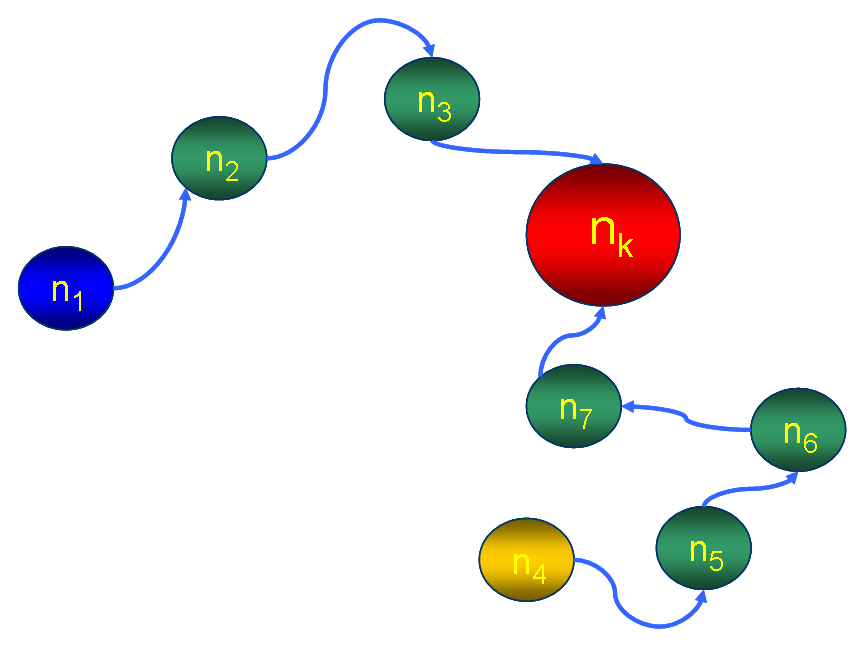
\includegraphics[width=6cm]{images/prize-sa}
    \caption{Paths and rewards in \textit{Spreading Activation}}
 \label{fig:prize-sa}
\end{figure}
  
  
\subsection{Refining Spreading Activation}
The whole configuration of the algorithm can be made by default but a customization
to a particular domain should be carried out by a domain expert taking into account the
specific issues of this domain and considering it as a new stage of 
the ontology o graph modeling process:

\begin{enumerate}
  \item The algorithm is highly coupled to the target ontology and domain. 
   Thus the adjustment and customization of the algorithm should be created or
  supervised by experts with domain knowledge. 
  \item The establishment of relation weights among concepts is
  the key point to customize \textit{SA} techniques. 
\end{enumerate}

Since \textit{SA} uses weights in relations  to calculate the activation
value of the concepts, different ``patterns'', see Tab.
\ref{guidingspreading}, have been identified to manage the direction of the spreading process.

\begin{table}[htb]

    \begin{tabular}{|p{3cm}|p{6cm}|p{3cm}|}
     \hline
      \textbf{Spread Direction} & \textbf{Definition} & \textbf{Key Relation} \\
        
	\hline
  	 Ascending& It seeks for the activation of concepts more generic than
the current. & ``superclass''\\
	\hline
  	 Descending& It seeks for the activation of concepts more specific than
the current. & ``superclass''\\
	\hline
  	 Nominal& It seeks for the activation of instances instead of concepts. &
``instance of'' \\
	\hline
  	 Crossing&  It seeks for the activation of concepts and instances connected
through a certain relation $\mathcal{R}$.  & $\mathcal{R}$ \\
     \hline

    \hline	
    \end{tabular}
    \caption{Patterns to manage the direction of SA.}
\label{guidingspreading}
\end{table} 

These control patterns can be put together in order to fit as much as possible the focus
and direction of the double process of activation and spreading.

\subsection{Design and implementation of ONTOSPREAD API}
ONTOSPREAD API is addressed by an open and extensible design applying
best practices on software design~\cite{Gamma,CoreJ2EEPatterns} and development~\cite{XP,Fowler1999}. 
The next basic objects to implement \textit{SA} technique have been identified.
\begin{itemize}

\item The \textit{Player} class handles the execution of the algorithm in a
      stepwise way. This is an application of the \textit{Iterator}
      design pattern to perform the activation and spreading processes. The state
      of the algorithm is captured in a separate class,
      \textit{OntoSpreadState} thus it is possible to serialize the
      state and back to a previous one.

\item The \textit{SA} process comprises of three sub-processes: \begin{inparaenum} 
    
 \item \textit{Preadjustement}: \textit{OntoSpreadPreAdjustment};
      \item \textit{Spreading} (activation and spreading) with constraints:
\textit{OntoSpreadRun}; and
      \item \textit{Postadjustment}:
\textit{OntoSpreadPostAdjustment}.\end{inparaenum}

Moreover, the process carries on the information about the knowledge base using the DAO
pattern thus the API is independent from the modeling language of the semantic network. Currently, OWL
and RDF are supported.
\end{itemize}

\begin{figure}[htb]
\centering
%	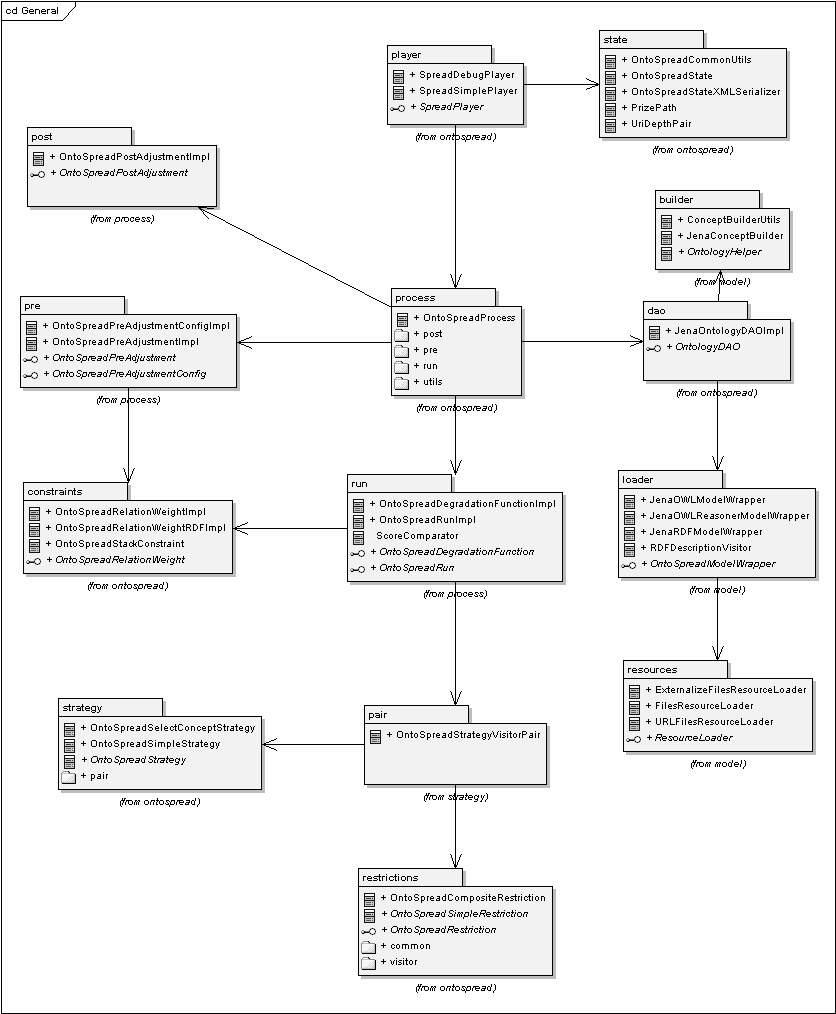
\includegraphics[width=8cm]{diagramas/general}
\caption{ONTOSPREAD Overview Diagram}
\label{fig:diagramas/general}
\end{figure}

\subsection{Designing the state of \textit{SA}}
The keypoint to design the algorithm lies in how and where
the information will be available at different iterations. Secondly, an unique entry point
to the state of the algorithm should be available trying to avoid
illegal accesses. This object stores the next information: \begin{inparaenum}\item Spread
concepts. \item Active concepts. \item Paths of activation. \item Concept to be
spread. \item Generic swap area (to share information among iterations). \end{inparaenum}

\subsection{Designing the restrictions of \textit{SA}}
The extensibility and flexibility of the algorithm is subjected to a good design
of the restrictions and their evaluation process. The next features and design patterns 
are used to design and implement the model of restrictions of SA:
\begin{itemize}
  \item Any restriction can be considered as a simple restriction and can be
evaluated to a boolean value.
  \item Conditions or actions in the algorithm can be comprised of several
restrictions.
  \item The extension points of the algorithm, included through a
\textit{Template Method} design pattern, are strategies to carry out an specific
action. Each strategy can be subjected to one or several restrictions.
\item Each restriction can be simple or comprised of others. \textit{Composite} pattern.
  \item Each action is an strategy. \textit{Strategy} pattern.
  \item A strategy implies one restriction (or a set of them) thus the strategy
is a client of the \textit{Composite} of restrictions.
  \item The evaluation of the restrictions to get their value (boolean) is
carried out through a \textit{Visitor} pattern that fits perfectly to evaluate and walk in
composite objects.
  \item The evaluation process consists on: apply the strategy that modifies the state
of the algorithm and assert this change of state by means of the restrictions applied
to this strategy.
\end{itemize}

\subsection{Development of ONTOSPREAD API and Supporting Tools}
The development of the API has been performed using Semantic Web and Java technologies
like: Jena\footnote{\url{http://jena.sf.net}} API, JAXB\footnote{\url{
http://java.sun.com/developer/technicalArticles/WebServices/jaxb/}}, 
Maven\footnote{\url{http://maven.apache.org}} o
Spring\footnote{\url{http://www.springframework.org/}}. Besides two tools are provided to test and debug different configurations
of the algorithm:

\begin{itemize}
 \item [ONTOSPREAD-TEST] It is a tool for the automatic execution and reporting
of batch tests. It provides an user-oriented framework to configure, combine and load several
configurations (e.g. restrictions, weights, initial concepts, etc.) for \textit{SA} and get results. A XML
vocabulary using XML-Schema and the \textit{Extensible Content Model} XML design
pattern has been defined to build the configuration of the \textit{SA} process.
 The designing of this vocabulary is oriented to be used with JAXB, this technology enables us 
automatically the processes of marshalling and unmarshalling Java classes providing an easy way to configure, 
load and serialize the different configurations and results. 

\item [ONTOSPREAD Inspector.] It is a graphical debugger of \textit{SA} algorithm 
using the graph library JpowerGraph\footnote{\url{http://jpowergraph.sf.net}} and
the SWT\footnote{\url{http://www.eclipse.org/swt/}} toolkit. It enables to configure, load, 
 run (one step or stepwise) and view the evolution of the semantic network 
 with the concepts (activated, spread, weights, relations, etc.).
\end{itemize}

Finally, a set of source code metrics using Eclipse\footnote{\url{http://www.eclipse.org}} and the 
metrics plugin\footnote{\url{http://metrics.sf.net/}} have been extracted to demonstrate and measure its 
quality. Table\ref{tabla:metricas-valores} presents these metrics that measures cohesion and coupling 
of the software.
   \begin{longtable}{|p{1cm}|p{4cm}|p{1cm}|p{1cm}|p{1cm}|p{1cm}|p{1.5cm}|}
        
        \caption{Source Code Metrics} \label{tabla:metricas-valores}\\
        \hline
        \multicolumn{7}{|c|}{\textbf{Source Code Metrics}}\\
        \hline
        \textit{ID} &  \textit{Def.} &  \textit{Total} &  \textit{Avg.}& 
\textit{Std. Dev.} & \textit{Max}& \textit{Scope} \\ \hline
        \endfirsthead
        \caption[]{Source Code Metrics (continue)}\\
        \hline
        \multicolumn{7}{|c|}{\textbf{Source Code Metrics}}\\
        \hline
        \textit{ID} & \textit{Def} & \textit{Total} &  \textit{Avg.}& 
\textit{Std.
        Dev.} & \textit{Max}& \textit{Scope} \\ \hline
        \endhead
        \hline
        \multicolumn{7}{|c|}{Continue $\ldots$}\\
        \hline
        \endfoot
        \hline
        \endlastfoot
		TLOC&Total Lines of Code.&5272&&&& \\ \hline
    		CA&Afferent Coupling.&&$6.524$&$10.545$&48&Package.\\ \hline
		RMD&Normalized Distance, $|RMA + RMI - 1 |$.&&$0.32$&$0.347$&1&Package. \\ \hline
		NOM&&$0.065$&$0.296$&3&Type. \\ \hline 
		RMI&Instability: $CE / (CA + CE)$&&$0.567$&$0.387$&1&Package. \\ \hline
		%NOF&Number of Atributtes.&147&$1.256$&$2.039$&12&Type. \\ \hline
		%NOP&Number of Packages.&42&&&& \\ \hline
		%MLOC&Method Lines of Code.&2661&$4.05$&$6.179$&88&Method. \\ \hline
		%WMC&Weighted methods per Class.&852&$7.282$&$6.859$&42&Type. \\ \hline
		%NORM&Number of Overriden Methods (no ``Object'' methods).&20&$0.171$&$0.419$&2&Type. \\ \hline
		%NSF&Number of Static Attributes.&58&$0.496$&$0.622$&$3$&Type. \\ \hline
		NBD&Nested Block Depth.&&$1.204$&$0.516$&4&Method. \\ \hline
		%NOM&Number of Methods.&594&$5.077$&$5.297$&33&Type.\\	\hline 
		LCOM&Lack of Cohesion of Methods (\textit{Henderson-Sellers}).&&$0.18$&$0.289$&$0.957$&Type.\\ \hline 
		VG&McCabe Cyclomatic Complexity.&&$1.297$&$0.735$&6&Method. \\ \hline
		RMA&Abstractness.&&$0.113$&$0.186$&0.667&Package. \\ \hline
		%NOI&Number of Interfaces.&11&$0.262$&$0.537$&2&Package. \\ \hline
		CE&Efferent Coupling.&&$1.976$&$1.282$&5&Package. \\ \hline
		%NC&11&$0.094$&$0.539$&5&N/A&Media y máximo por tipo. \\ \hline
		DIT&Depth of Inheritance Tree.&&$1.607$&$0.915$&4&Type. \\ \hline
    	 \hline
        \end{longtable}      

All of these values are in the default range defined in the plugin thus the quality of the source code 
with the desired feautures of \textit{high cohesion} and \textit{low coupling} are assured.
\section{Evaluation of ONTOSPREAD API}
The validation of the algorithm depends on the configuration of the activation and spreading processes to
fit it to the different domain issues. SA is determined by the target semantic network and therefore
the defined domain knowledge (concepts and relations) is the key part to adjust its behavior. On the other
hand, taking into account that the activation and spreading is guided by the weights of relations their specification 
is fundamental to get the desired outputs. The methodology to test the implementation
of the algorithm is subjected to these conditions but a step-wise refinement method can be outlined:
\begin{enumerate}
  \item Use a well-known semantic network (ontology, etc.): concepts and relations.
  \item Define a potential set of initial concepts ($\Phi$) and their initial activation value (usually $1.0$).
  \item Specify the weights of the relations to that domain knowledge.
  \item Combine the different restrictions provided by the framework.
  \item Select the degradation function.
  \item Add the reward techniques to increase the activation value of certain nodes.
  \item Try to evaluate new activation functions for their further implementation.
  \item Repeat these steps until getting the most appropriated set of output concepts to that domain knowledge.
\end{enumerate}

To apply this methodology, the GALEN and SNOMED CT~\footnote{The OWL version of SNOMED CT has been generated using ``Simple SNOMED Module Extractor'' provided by the OWL Research Group at Manchester University:~\url{http://owl.cs.manchester.ac.uk/snomed/}. Other tests 
have been carried out using the OWL version of SNOMED CT provided by the IHTSDO.} ontologies have been selected. 
They are well-known and referenced ontologies in the biomedicine domain and they are widely used in reasoning and decision support processes. 
The design of the experiment depends on: the ontology, the weights of relations, the set of initial concepts, 
the set of restrictions, the degradation function and the extensions to reward nodes. 
In the case of GALEN, the set of initial concepts ($\Phi$) with an initial value $1.0$ is: 
``\#AdvancedBreastCancer'' and ``\#NAMEDSymptom''. The weights of the 
relations are fixed to a default value of $1.0$. On the other hand, the set of initial concepts ($\Phi$) with an initial value $1.0$ 
in SNOMED-CT is: ``\#Articular\_cartilage\_of\_lunate'' and ``\#Articular\_tissue\_sample''

The refinement of the algorithm will enable us to get
a set of output concepts similar to the process that a brain will do. The degradation functions
and the reward technique will be alternatively combined checking the output of the algorithm. 

\begin{table*}[!h]
\renewcommand{\arraystretch}{1.3}
\begin{center}
\begin{tabular}{|p{3cm}|p{1.5cm}|p{1.5cm}|p{1.5cm}|p{1.5cm}|p{1.5cm}|p{1.5cm}|}
\hline
        \textbf{Config \& Stats/Test}&$T_1$&$T_2$&$T_3$&$T_4$&$T_5$&$T_6$\\ \hline
        \hline
        Minimum activation value $N_{\min}$ &$1.0$ &$1.0$ &$1.0$ &$1.0$&$1.0$&$1.0$ \\ \hline
	Maximum number of spread concepts $\mathbb{M}$&$50$ &$50$ &$10$ &$10$&$50$&$50$\\ \hline
	Minimum number of spread concepts $\mathbb{M_{\min}}$&$20$ &$20$ &$5$ &$5$&$20$&$20$  \\ \hline
	Output Degradation $O_j$ & $h_1$ &$h_2$ &$h_1$ &$h_2$&$h_1$&$h_2$\\ \hline
	Reward (No,Yes) &N &N &N &N&Y&Y\\ \hline
	\hline
	Context of activation $\mathbb{D}_{com}$&\multicolumn{6}{|c|}{DEFAULT} \\ \hline
	Activated Nodes &$62$ &$79$ &$15$ &$15$&$62$&$79$ \\ \hline
	Spread Nodes &$20$ &$20$ &$5$ &$5$&$20$&$20$ \\ \hline
	Highest activation value &$7.5$ &$3.9896$ &$1.5$ &$1.90$&$7.5$&$3.9896$\\ \hline
	Deepest spread path &$10$ &$16$&$2$ &$2$&$10$&$16$\\ \hline
	Concepts (name:value) & NAMED Symptom: $7.5$, Primate: $2.28$ &Multi Cellular Eukaryota: $3.9896$, Opis thokonts: $3.9885$ &NAMED Symptom: $1.5$, Advanced Breast Cancer: $2.28$ &NAMED Symptom: $1.90$, Advanced Breast Cancer: $1.90$&NAMED Symptom: $7.5$, Primate: $2.28$&Multi Cellular Eukaryota: $3.9896$, Opis thokonts: $3.9885$ \\ \hline
	Time (msec.) & $9$ &$8$ &$2$ &$3$&$11$&$12$ \\ \hline
\end{tabular}
  \caption{Configuration and statistics of results after the execution and refinement of SA over the Galen ontology.}
  \label{tabla:test-restricciones}
  \end{center}
\end{table*} 

After the execution of the different configurations, see Tab.~\ref{tabla:test-restricciones} and Tab.~\ref{tabla:test-snomed}, 
some statistics have been extracted out of the results. 
The main differences between the tests lies in the number of activated nodes and their activation values due to the restrictions that guide the evolution
of the algorithm through the graph and the structure of the ontologies. 
It is also remarkable that the reward of paths, in this case, does not imply changes in the output set. This situation demonstrates 
that a depth knowledge of the semantic network is needed to take advantage of the SA extensions. Nevertheless the output of the
algorithm helps us to establish a set of weighted resources that can be used to retrieve documents, make recommendations or search in 
large databases with enriched queries.


\begin{table*}[!h]
\renewcommand{\arraystretch}{1.3}
\begin{center}
\begin{tabular}{|p{3cm}|p{1.5cm}|p{1.5cm}|p{1.5cm}|p{1.5cm}|p{1.5cm}|p{1.5cm}|}
\hline
        \textbf{Config \& Stats/Test}&$T_1$&$T_2$&$T_3$&$T_4$&$T_5$&$T_6$\\ \hline
        \hline
        Minimum activation value $N_{\min}$ &$1.0$ &$1.0$ &$1.0$ &$1.0$&$1.0$&$1.0$ \\ \hline
	Maximum number of spread concepts $\mathbb{M}$&$50$ &$50$ &$10$ &$10$&$50$&$50$\\ \hline
	Minimum number of spread concepts $\mathbb{M_{\min}}$&$20$ &$20$ &$5$ &$5$&$20$&$20$  \\ \hline
	Output Degradation $O_j$ & $h_1$ &$h_2$ &$h_1$ &$h_2$&$h_1$&$h_2$\\ \hline
	Reward (No,Yes) &N &N &N &N&Y&Y\\ \hline
	\hline
	Context of activation $\mathbb{D}_{com}$&\multicolumn{6}{|c|}{DEFAULT} \\ \hline
	Activated Nodes &$136$ &$76$ &$16$ &$16$&$136$&$76$ \\ \hline
	Spread Nodes &$20$ &$20$ &$5$ &$5$&$20$&$20$ \\ \hline
	Highest activation value &$2.16$ &$9.49$ &$1.5$ &$1.85$&$4.14$&$13.68$\\ \hline
	Deepest spread path &$10$ &$7$&$3$ &$3$&$10$&$16$\\ \hline
	Concepts (name:value) & Upper extremity part: $2.16$, Articular cartilage of wrist joint: $1.66$ &Structure of radioulnar joint: $9.49$, Inferior radioulnar joint structure: $8.5$ &Articular cartilage of lunate: $1.5$, Wrist region structure: $1.0$ &Articular cartilage of lunate: $1.85$, Joint structure of wrist and/or hand: $1.0$&Upper extremity part: $4.14$, Joint structure of wrist and/or hand: $1.2$&Wrist joint structure: $13.68$, Inferior radioulnar joint structure: $8.5$ \\ \hline
	Time (msec.) & $36$ &$17$ &$3$ &$4$&$42$&$17$ \\ \hline
\end{tabular}
  \caption{Configuration and statistics of results after the execution and refinement of SA over the SNOMED CT ontology.}
  \label{tabla:test-snomed}
  \end{center}
\end{table*} 


\section{Conclussions and Future Work}
FIXME: Revisar

This work provides a configurable and extensible API to support the SA technique. It allows
the configuration of restrictions and their combination to get
the most accurate set of output concepts. One of the features that
turns SA to a widely accepted algorithm lies in its flexibility 
but some disadvantages are also presented: the adjusting and refinement of
the restrictions and the weights of the relations, the selection of the
degradation function or the establishment of reward functions. This API
minimizes these advantages with an extensible framework that can be
applied to different scenarios like digital libraries in particular
biomedicine, e-procurement, e-health, etc. providing enriched services
of annotation, searching or recommendation.

The main improvement in the algorithm consists on the flexibilization of
the refinement methodology. An automatic learning algorithm to create SA configurations
according to ontologies should be developed. Thus, the training stage of SA could generate
the best configuration for a specific domain. The algorithm could optimize the selection 
of input parameters like the weights of the relations, the degradation functions 
or the combination of restrictions. Beside new mesaures related to instances such as `Cluster
Measure'', ``Specifity Measure'' or both could be used in the process of activation/spreading.
Also the selection of the next node to spread is based on a ``first
better'' strategy (if two nodes have the same activation value) because of this fact
other selection strategies should be implemented.

\subsection*{Acknowledgements}
ONTOSPREAD API has been initially developed in BOPA~\cite{bopaEstonia} project that is
one of \textit{Semantic Web Use Cases and Case
Studies}\footnote{\url{http://www.w3.org/2001/sw/sweo/public/UseCases/CTIC/}}
collected by W3C. Currently it is being applied to the process of searching
public procurement notices in the ``10ders Information Services''\footnote{\url{http://rd.10ders.net}} project, partially funded by 
the Spanish Ministry of Industry, Commerce and Tourism (TSI-020100-2010-919) 
and the European Regional Development Fund (EFDR), leaded by ``Gateway Strategic Consultancy Services''\footnote{\url{http://gateway-scs.es/}} 
and developed in cooperation with ``Exis TI''\footnote{\url{http://www.exis-ti.com/}}  and WESO Research Group.

% \section{Introduction}
% 
% \textit{Spreading Activation} techniques (hereafter \textit{SA}) rise in the
% Psychology area, as result of human memory researches~\cite{AndersonTheory} and
% more specifically, in the search of ways to exploit human knowledge
% representation:
% \begin{inparaenum} \item Procedural semantics.
% \item Semantic features. \item Semantic Networks\footnote{From Psychology point of
% view.}.\end{inparaenum}
% 
% 
% In the Semantic Web domain and regarding the use of ontologies as knowledge
% bases, they could be taken as a kind of semantic network that models concepts and their relationships using
% a certain sort of logics, e.g. Description Logics (DLs). In some sense,
% ontologies capture a domain knowledge and express it as a logic structure, just
% as the human memory does.
% 
% Knowledge representation using a set of concepts related fits to real world.
% Concepts can express overall relations and data but also particular domain
% knowledge. That's why it is relevant provide an useful method to obtain sets of related
% concepts efficiently and automatically. Usually, the methods to explore knowledge bases can be split into: \begin{inparaenum} efficient search algorithms (based on \textit{Brand and Bounch}) in semantic networks or graphs. \item Neural networks~\cite{Chen95}\end{inparaenum}. \textit{SA}
% techniques provide us a method to explore semantic networks as an iterative way
% (performance oriented) and can be applicable to different problems:
% Information or Document retrieval. Our main goal is applied these techniques to
% ontologies, getting a new method to rank the concepts and their relations
% according to a query.
% 
% \subsection{Related work}
% The use of \textit{SA} as algorithm to explore graphs is not a new approach and
% since 80's\cite{Scott1981} appeared the first works naming it. The
% main use was focused in Document~\cite{Cui03,Kobayashi00,turtle91inference,2917612} and Information
% Retrieval~\cite{Agosti1993,Cohen1987,Baeza99} altough the appearance/born of Internet Spreading
% Activation has been used in retrieve resources from the network:
% hypertext~\cite{Agosti1993} or multimedia with a real trust measurement~\cite{ziegler-lausen-04}. On other hand, these techniques has been used in semantic search based on hybrid approaches~\cite{RochaSA04,XueHYZCM04}, user query expansion~\cite{767402} combining metadata and user information or improve web data annotations~\cite{GelgiVD05}.
% 
% \subsection{Main contribution}
% 
% The aim of this paper is to introduce the application and refining \textit{SA}
% tecniques in the activation of concepts defined in the ontologies and the
% algorithm design through a generic Java API, called OntoSpread that handles the
% process of activation and spread concepts. Furthermore, OntoSpread \footnote{\url{http://sf.net/projects/ontospread}} has
% been developed as an open source project hosts in Sourceforge under LGPL license
% to easy its use and future contributions.
% 
%
% \section{OntoSpread: the design of an API for Spreading Activation}
% 
% Our Spreading Activation API focuses on an open design, best
% practices~\cite{XP,Fowler1999} and makes extensive use of design
% patterns~\cite{Gamma,CoreJ2ee}. We have identified the next basic objects need
% to implement \textit{SA} techniques.
% 
% \begin{itemize}
% 
% \item The \textit{Player} class handles the execution of the algorithm in a
%       stepwise way. This is an application of the \textit{Iterator}
%       design pattern to the activation and spreading processes. The state
%       of the algorithm is captured in a separate class,
%       \textit{OntoSpreadState}, so it is possible to serialize the
%       status and to move backwards.
% 
% \item The \textit{SA} process comprises three sub-processes: \begin{inparaenum} 
%     
%  \item \textit{Preadjustement}: \textit{OntoSpreadPreAdjustment};
%       \item \textit{Spreading} (activation and spreading) with constraints:
% \textit{OntoSpreadRun}; and
%       \item \textit{Postadjustment}:
% \textit{OntoSpreadPostAdjustment}.\end{inparaenum}
% Moreover, the process has information about the knowledge base using a DAO
% pattern so the API is independent from the modelling language. Currently, OWL
% and RDF are supported. Although we have brought forward the use of another
% languages as SKOS-Core or WSML, providing the need operations to extract the
% information about concepts and their relations.
% \end{itemize}
% 
% 
% 
% %\begin{figure}[htb]
% %\centering
% %	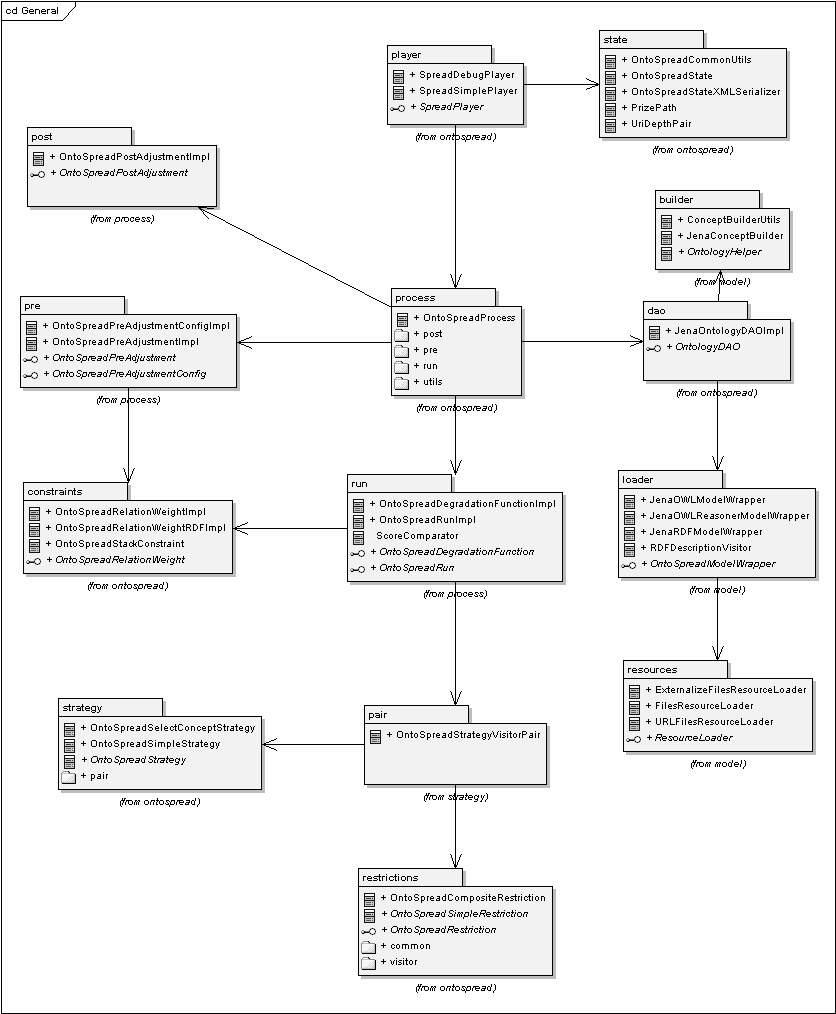
\includegraphics[width=8cm]{diagramas/general}
% %\caption{Diagrama general}
% %\label{fig:diagramas/general}
% %\end{figure}
% 
% 
% \subsection{Designing of the state for \textit{SA}}
% 
% In the first one, the keypoint to design the algorithm falls in how and where
% the information will be available at different iterations. Secondly, we want to
% provide an only one access point to the state of the algorithm trying to avoid
% weak states and providing an easy way for supportting. 
% This object stores the next information: \begin{inparaenum}\item Spread
% concepts. \item Active concepts. \item Paths of activation. \item Concept to be
% spread. 
% \item Generic swap area (to share information). \end{inparaenum}
% 
% \subsection{Designing of restrictions for \textit{SA}}
% The extensibility and flexibility of the algorithm is subjected to a good design
% of the restrictions and the procedure of their evaluation. The next features and design patterns are used to guide the model of restrictions for SA:
% 
% \begin{itemize}
%   \item Any restriction can be considered as a simple restriction and can be
% evaluated to a boolean value.
%   \item Conditions or actions in the algorithm can be composed of several
% restrictions.
%   \item The extension points of  the algorithm, included through a
% \textit{Template Method} design pattern, are strategies to carry out an specific
% action. Each strategy can be subjected to one or several restrictions.
% \item Each restriction can be simple or composed by other ones.
% \textit{Composite} pattern.
%   \item Each action is an strategy. \textit{Strategy} pattern.
%   \item One strategy entails one restriction (or set of them) so the strategy
% seems a client of the \textit{Composite} of restrictions.
%   \item The evaluation of the restrictions to get their value (boolean) is
% carried out
%   through a \textit{Visitor} pattern that fits perfectly to do the evaluation of
% composite objects.
%   \item The evaluation process consists on:
%   \begin{inparaenum}
%   \item Apply the strategy, this step modifies thc execution and reporting
% of batch tests. It provides a framework to configure, combine and load several
% configurations for \textit{SA} and obtain results. We have designed a XML
% vocabulary using XML-Schema and the \textit{Extensible Content Model} xml design
% pattern to build the configuration of the \textit{SA} process. The designing of
% this vocabulary is oriented to be used with JAXB, this technology allow us the
% generation of Java classes automatically and we can marshalling and
% unmarshalling objects providing a good way to configure, load and serialize
% different configurations. The main goal to define a new XML vocabulary can be
% arguable, but this vocabulary is not a new XML to be interchanged among
% applications, we only use inside OntoSpreadTest and to provie state of the algorithm. 
%   \item Validate the changes, the restricctions assert the
% changes.\end{inparaenum}
% 
% \end{itemize}
% 
% 
% 
% %\begin{figure}[htb]
% %\centering
% %	\includegraphics[width=8cm]{diagramas/restricciones}
% %\caption{Diagrama general de restricciones \textit{SA}}
% %\label{fig:diagramas/restricciones}
% %\end{figure}
% 
% 
% \subsection{OntoSpread development}
% 
% The development of the API has been carried out using Semantic Web tecnologies
% and web development tecnology as: Java programming language, 
% Jena\footnote{\url{http://jena.sf.net}} API, 
% JAXB\footnote{\url{
% http://java.sun.com/developer/technicalArticles/WebServices/jaxb/}}, 
% Maven\footnote{\url{http://maven.apache.org}} o
% Spring\footnote{\url{http://www.springframework.org/}}. We have built a
% graphical viewer and debugger,
% \textit{OntoSpread Inspector}, using the graph library
% JpowerGraph\footnote{\url{http://jpowergraph.sf.net}} and
% SWT\footnote{\url{http://www.eclipse.org/swt/}}.
% 
% \subsubsection{Source code metrics}
% 
% We have extracted, using Eclipse\footnote{\url{http://www.eclipse.org}} and the
% metrics plugin\footnote{\url{http://metrics.sf.net/}},  
% some source code metrics (only for OntoSpread API) to show and mesaure its
% quality. We present the most meaningful source code metrics, 
% see Table \ref{tabla:metricas-valores}, based on the definitions
% in~\cite{229953}. These metrics measures cohesion and coupling of the software and can be useful
% to decide if the code is well structured.
% 
%    \begin{longtable}{|p{1cm}|p{4cm}|p{1cm}|p{1cm}|p{1cm}|p{1cm}|p{1.5cm}|}
%         
%         \caption{Source Code Metrics} \label{tabla:metricas-valores}\\
%         \hline
%         \multicolumn{7}{|c|}{\textbf{Source Code Metrics}}\\
%         \hline
%         \textit{ID} &  \textit{Def.} &  \textit{Total} &  \textit{Avg.}& 
% \textit{Std. Dev.} & \textit{Max}& \textit{Scope} \\ \hline
%         \endfirsthead
%         \caption[]{Source Code Metrics (continue)}\\
%         \hline
%         \multicolumn{7}{|c|}{\textbf{Source Code Metrics}}\\
%         \hline
%         \textit{ID} & \textit{Def} & \textit{Total} &  \textit{Avg.}& 
% \textit{Std.
%         Dev.} & \textit{Max}& \textit{Scope} \\ \hline
%         \endhead
%         \hline
%         \multicolumn{7}{|c|}{Continue $\ldots$}\\
%         \hline
%         \endfoot
%         \hline
%         \endlastfoot
% 		TLOC&Total Lines of Code.&5272&&&& \\ \hline
%     		CA&Afferent Coupling.&&$6.524$&$10.545$&48&Package.\\ \hline
% 		RMD&Normalized Distance, $|RMA + RMI - 1 |$.&&$0.32$&$0.347$&1&Package. \\ \hline
% 		NOM&&$0.065$&$0.296$&3&Type. \\ \hline 
% 		RMI&Instability: $CE / (CA + CE)$&&$0.567$&$0.387$&1&Package. \\ \hline
% 		%NOF&Number of Atributtes.&147&$1.256$&$2.039$&12&Type. \\ \hline
% 		%NOP&Number of Packages.&42&&&& \\ \hline
% 		%MLOC&Method Lines of Code.&2661&$4.05$&$6.179$&88&Method. \\ \hline
% 		%WMC&Weighted methods per Class.&852&$7.282$&$6.859$&42&Type. \\ \hline
% 		%NORM&Number of Overriden Methods (no ``Object'' methods).&20&$0.171$&$0.419$&2&Type. \\ \hline
% 		%NSF&Number of Static Attributes.&58&$0.496$&$0.622$&$3$&Type. \\ \hline
% 		NBD&Nested Block Depth.&&$1.204$&$0.516$&4&Method. \\ \hline
% 		%NOM&Number of Methods.&594&$5.077$&$5.297$&33&Type.\\	\hline 
% 		LCOM&Lack of Cohesion of Methods (\textit{Henderson-Sellers}).&&$0.18$&$0.289$&$0.957$&Type.\\ \hline 
% 		VG&McCabe Cyclomatic Complexity.&&$1.297$&$0.735$&6&Method. \\ \hline
% 		RMA&Abstractness.&&$0.113$&$0.186$&0.667&Package. \\ \hline
% 		%NOI&Number of Interfaces.&11&$0.262$&$0.537$&2&Package. \\ \hline
% 		CE&Efferent Coupling.&&$1.976$&$1.282$&5&Package. \\ \hline
% 		%NC&11&$0.094$&$0.539$&5&N/A&Media y máximo por tipo. \\ \hline
% 		DIT&Depth of Inheritance Tree.&&$1.607$&$0.915$&4&Type. \\ \hline
%     	 \hline
%         \end{longtable}      
% 
% 
% All of these values are in the default range defined in the plugin thus we can
% assure the quality of the source code with the desired feautures of \textit{high
% cohesion} and \textit{low coupling}.
% 		
% 
% \subsection{OntoSpread tools}
% 
% The development of a new API requires a test bed to ensure: \begin{inparaenum} 
% \item the functional requirements of the API, we must check if the algorithm
% implements the \textit{SA} model. Black box tests. \item White Box tests, we
% have made 50 unit tests.
%                                                             \end{inparaenum} 
% However, these tests are programmer oriented and we want to provide tools that
% can be used to test the API with nontechnical people. Therefore, we have
% designed and implemented two different tools:
% \begin{description}
% 
%  \item [OntoSpreadTest.] it is a tool for the automatic execution and reporting
% of batch tests. It provides a framework to configure, combine and load several
% configurations for \textit{SA} and obtain results. We have designed a XML
% vocabulary using XML-Schema and the \textit{Extensible Content Model} xml design
% pattern to build the configuration of the \textit{SA} process. The designing of
% this vocabulary is oriented to be used with JAXB, this technology allow us the
% generation of Java classes automatically and we can marshalling and
% unmarshalling objects providing a good way to configure, load and serialize
% different configurations. The main goal to define a new XML vocabulary can be
% arguable, but this vocabulary is not a new XML to be interchanged among
% applications, we only use inside OntoSpreadTest and to provide an easy way to
% handle XML configurations in Java through JAXB. E.g. the XML vocabulary belong
% us configure restrictions as an iterative model, Fig. \ref{example-iterator}.
% Summarizing, OntoSpreadTest is an interpreter of our XML vocabuluary.
% 
% \begin{figure}
% \lstset{language=XML}
% \begin{lstlisting}
% <restriction xsi:type="activationRestriction">
%  <config>
%    <init>0.3</init>
%    <step>0.1</step>
%    <stop>1</stop>
%  </config>  
% </restriction>
% \end{lstlisting}
% \caption{Configuring a restriction.}
% \label{example-iterator}
% \end{figure}
% 
% \item[OntoSpread Inspector.] It is a graphical debugger,
%  of \textit{SA} algorithm. It follows the idea of an
%  inspector inside an ide and belongs: configure, load, run (one step or stepwise)
%  and view the evolution of the semantic network with the concepts (activated,
%  spread, weights, relations, etc.). The main goal of this tool is provide an
%  environment to debug, inspect and change the state of the algorithm.
% 
% \end{description}
%  
% \subsection{Working with OntoSpread API}
% 
% \subsubsection{BOPA}\label{proyecto:bopa}
% OntoSpread API has been integrated in BOPA~\cite{bopaEstonia} project that is
% one of \textit{Semantic Web Use Cases and Case
% Studies}\footnote{\url{http://www.w3.org/2001/sw/sweo/public/UseCases/CTIC/}}
% collected by W3C.\textit{SA} techniques are used as part of an hybrid search
% process, see Fig~\ref{fig:sa-search}, they are in charge of the subprocess of
% query expansion taking as set of initial concepts the concepts retrieved from
% the user query.
%  \begin{figure}[h]
%  \centering
%     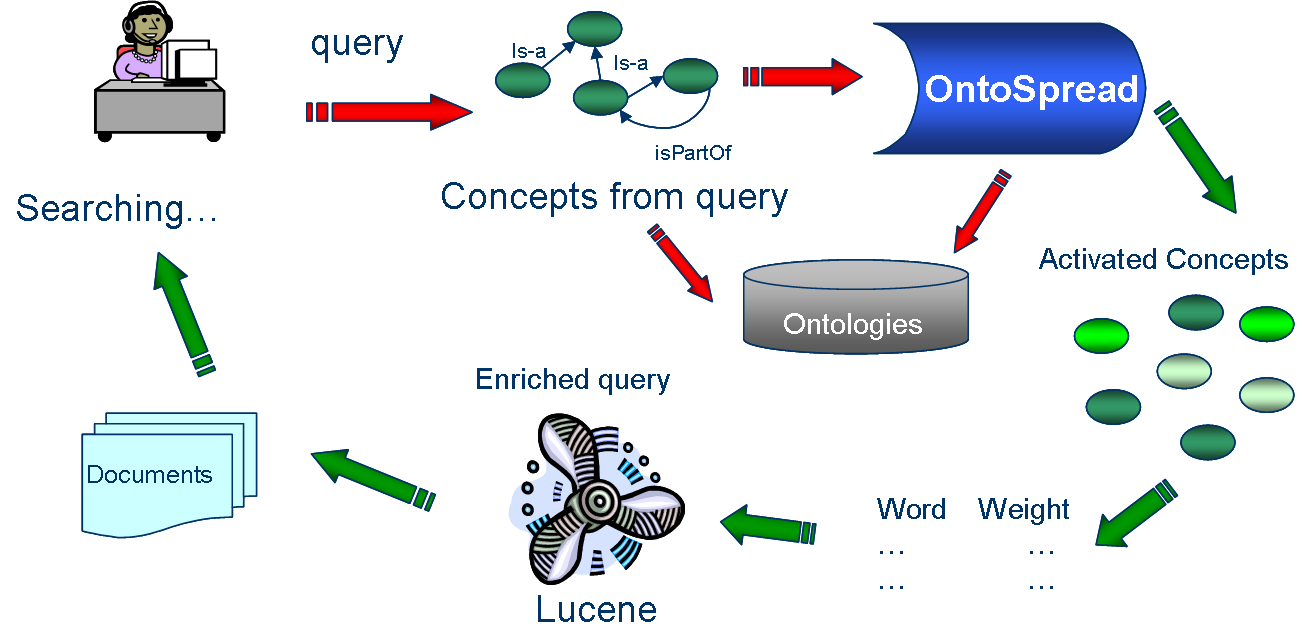
\includegraphics[width=10cm]{images/sa-search}
%     \caption{Applying \textit{Spreading Activation} in BOPA}
%  \label{fig:sa-search}
% \end{figure}
% 
% 
% \subsubsection{DBPedia}
% FIXME
%   
% 
% \section{Conclussions and future work}
% 
% \textit{SA} techniques are a combination of restrictions that provide us a
% method to build a set of ranked concepts from a conceptual network as well as a
% human memory does. The application of \textit{SA} is very suitable for a large
% number of scenarios and use cases providing a method to get ``artificial
% suggestions'' closed to human. If we would have to resume \textit{SA} techniques
% in one word, is \textit{flexibility}.
% 
% \begin{enumerate}
% \item Flexibility, extensibily and modularity.
% \item Several scenerarios and use cases to be applied.
% \item The adjusting and refining of the algorithm is a task for domain experts.
% \item It is similar to  a ``helper'' (domain expert).
% \end{enumerate}
% 
% The main goal to improve an algorithm so many flexible as \textit{SA} will be
% adjust and refine its 
% operation for the problem of activation and spread concetps in ontologies. The
% keypoints could be:
% \begin{itemize}
%  \item An automatic learning algorithm to build configurations for OntoSpread
% according to ontologies. Thus, the training of this algorithm could generates
% the best configuration for a specific domain. The algorithm could optimize all
% of the parameters in the algorithm: weights of the relations, activation
% function (parameter of degradation) or the combine of restrictions.
% \item Use of mesaures related to instances~\cite{RochaSA04} as `Cluster
% Measure'', ``Specifity Measure'' or both in the process of activation/spreading.
% \item Development of techniques to select\footnote{Currently, we use ``first
% better''.} the next concept to be spread based on metaheuristics or Tabu
% search~\cite{Glover1990,Gendreau}.
% \item Study and application of \textit{SA} as helper of semi automatic methods
% as mapping~\cite{Bruijin2006} between ontologies or tagging with folksonomies.
% \end{itemize}
% 
% 
%\nocite{*}

% Formal\cite{Scott1981,Cohen1987}
% Data mining\cite{paper:troussov:2008}
% Information Retrieval\cite{SpreadingActivationIR,Helmut2004,Agosti1993,Grinberg:2011:ASA:1940632.1940674}
% Concept exploration\cite{Qiu93} and ontologies\cite{Chen95,DBLP:journals/cogsr/KatiforiVD10,DBLP:journals/ijsc/DixKLVS10,liu_et_al_2005}
% Annotations\cite{GelgiVD05,Chen:2007:PSA:1780653.1780702}
% Tagging\cite{labraTagging2007}
% Web Search\cite{XueHYZCM04}
% Natural Language\cite{Tsatsaronis:2007:WSD:1625275.1625555}
% Recommendations\cite{citeulike:3779904,gouws-vanrooyen-engelbrecht:2010:CCSR}
% Semantic Search\cite{conf-sofsem-Suchal08,Wolverton94retrievingsemantically,Schumacher+2008search,bopaEstonia,RochaSA04,LabraWesoNet}
% Ing. software\cite{CoreJ2EEPatterns}


\bibliographystyle{plain}
% %\bibliographystyle{unsrt}
% %\bibliographystyle{acm}
\bibliography{bib/references}
% \renewcommand{\bibname}{References}
\end{document}
